\chapter{Аналитический раздел}

\section{Gameplay игры}

Игра <<Pinball для двух игроков>> имеет 2 режима работы:
\begin{enumerate}
\item Два пользователя на одной клавиатуре.
\item Пользователь против бота.
\end{enumerate}

Экран игры разбит на два поля. У каждого игрока - своё поле для игры в Pinball. Взаимодейсвтие игроков заключается в перебрасывании шаров через отверстие в стене, разделяющее два поля. Поражение наступит либо при утере 5 шаров, либо при отставании в счете от соперника более чем на 5000000 очков. На рисунке ~\ref{image:gameplay} показан gameplay игры. 

\begin{figure}[h]
  \centering
  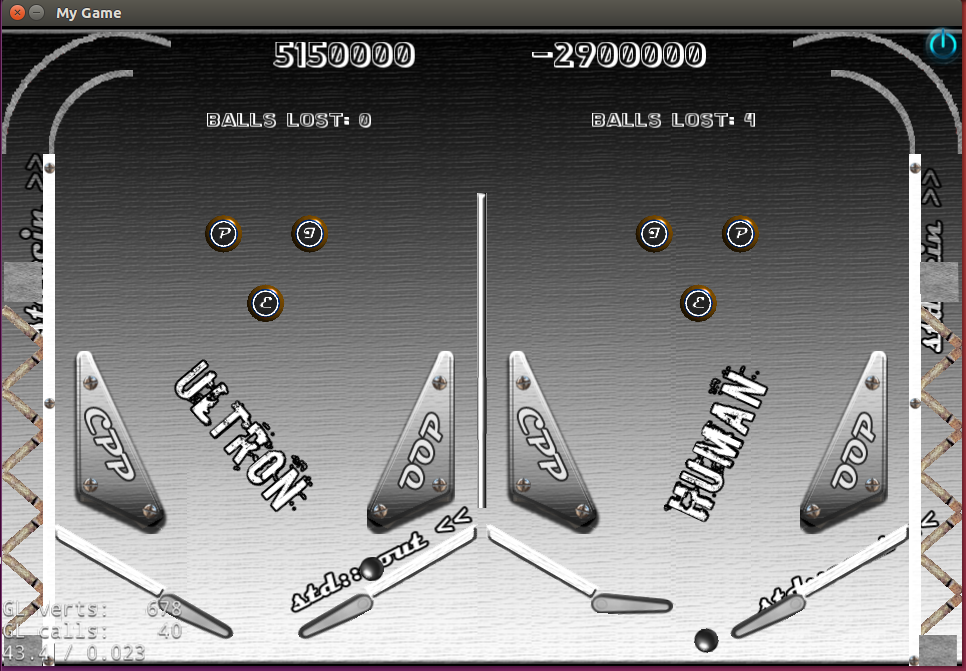
\includegraphics[width=\textwidth]{gameplay.png}
  \caption{Gameplay игры.}
  \label{image:gameplay}
\end{figure}

\section{Передаваемые данные}

Для того, чтобы создать сетевой мультиплеер для данной игры необходимо изучить, какие данные необходимо передавать между клиентами. Между двумя игроками будут передаваться сведения о следующих объектах:
\begin{enumerate}
\item шары;
\item пружина;
\item рычаги.
\end{enumerate}

В связи со спецификой игры, для каждого объекта будут передавться следующие данные:
\begin{enumerate}
\item шар:
	\begin{enumerate}
	\item координата X;
	\item координата Y;
	\item скорость по X;
	\item скорость по Y;
	\item угол поворота.
	\end{enumerate}	
\item пружина:
	\begin{enumerate}
	\item координата Y;
	\end{enumerate}
\item рычаг:
	\begin{enumerate}
	\item какой рычаг (левый или правый);
	\item флаг активации;
	\end{enumerate}
\end{enumerate}

Дополнительная информация, необходимая для игроков:
\begin{enumerate}
\item счет;
\item имя;
\end{enumerate}

\section{Требования к серверу}

\begin{enumerate}
\item возможность одновременной игры более 1 пары игроков;
\item поиск соперника происходит простым ожиданием первого подключившегося игрока;
\item запись лога событий.
\end{enumerate}

